\documentclass[relatorio.tex]{subfiles}
\begin{document}
Nesta última fase proposta pelo enunciado do trabalho prático foi necessário a 
criação de novas classes, sendo estas acrescentadas com base na estrutura realizada
na primeira fase. As novas classes foram criadas com base nos novos elementos do ficheiro
XML, nomeadamente, \textit{texture}, \textit{color} e \textit{lights}, mantendo assim a 
responsabilidade de leitura do XML para a classe responsável por manipular estes elementos.

Apesar de não existir \textit{normals} no ficheiro XML, foi criada a classe \textit{normals},
responsável pela leitura das normais presentes no ficheiro .3d criado pelo \textit{generator}.

\begin{landscape}
    \begin{figure}
        \centering
        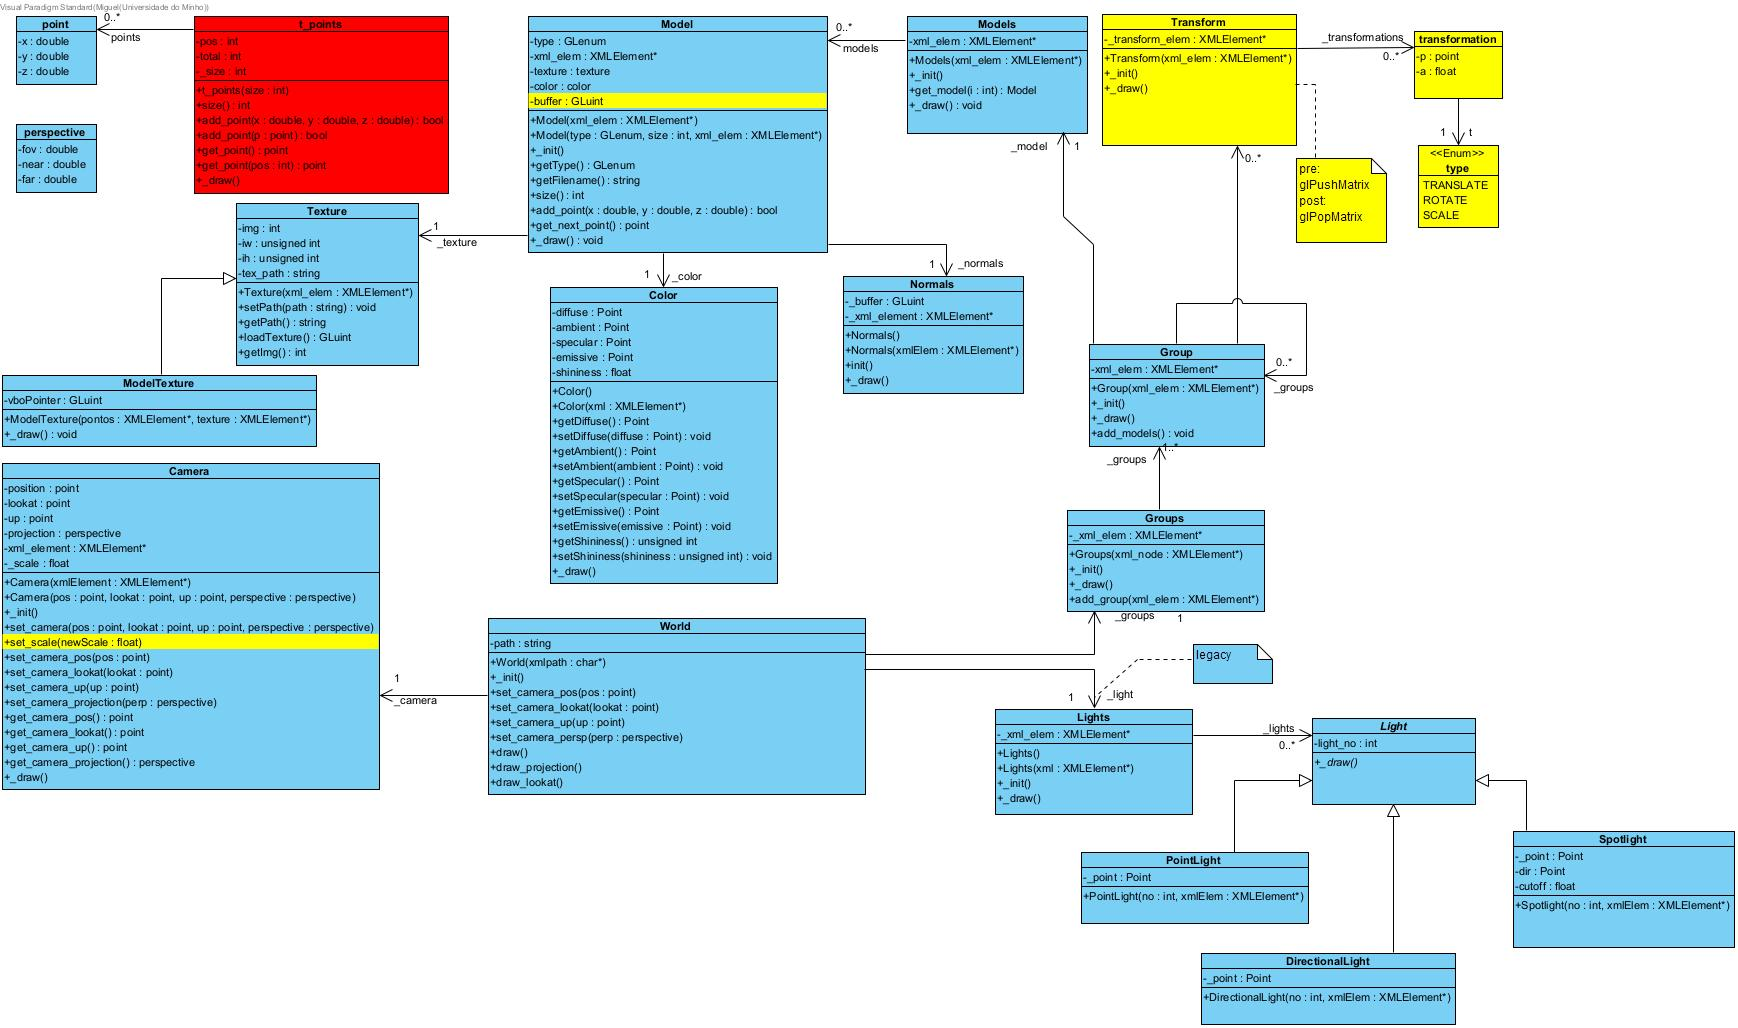
\includegraphics[width=\linewidth]{assets/classe.jpg}
        \caption{Diagrama de classes} \label{fig:dig_classes}
    \end{figure}
\end{landscape}

\subsection{Luzes}
Para tratar das diferentes tipos diferentes de luzes foram criadas foram criadas
três subclasses da classe abstrata \textit{Light}:
\begin{itemize}
    \item \textit{DirectionalLight}
    \item \textit{PointLight}
    \item \textit{Spotlight}
\end{itemize}

Em que a classe abstrata tem como argumento o número da luz, e as subclasses os
parâmetros necessários para a sua ativação.

A classe \textit{Lights} que é classe agregadora de todas as luzes do modelo e a
responsável por processar o elemento \textit{lights} do ficheiro XML\dots

Todas as luzes são inicializadas com os valores \textit{default} de luz ambiente,
difusa e especular semelhantes à \textbf{LIGHT0}.
Apenas difere na luz ambiente, pois utiliza-se um valor diferente de $0$ 
para haver alguma luminosidade da parte de trás dos objetos, obtendo uma 
melhor simulação da realidade.

No seguimento da ativação das luzes, tornou-se necessário a ativação das normais com
recurso a \textbf{VBO}s.

Assim, com recurso a uma classe criada para o efeito, designada \textbf{Normals},
foi possível instituir a utilização de normais em cada modelo.
A estratégia utilizada consistiu em ler o ficheiro XML, gerar um \textit{buffer}
na gráfica, efetuar o seu binding e popular com pontos.
Posteriormente, ao realizar o \textbf{rendering}, efetua-se a verificação se existe
alguma textura associada ao modelo e, caso exista, é executado o método \textit{\_draw}
da classe \textit{Normals}.

\subsection{Cores}
A classe \textit{Color} tem como argumentos as 5 componentes da luz,
que são inicializadas por defeito com os valores passados pela equipa docente
no enunciado do trabalho. 

\inputminted[firstline=19, lastline=25]{cpp}{../../Color.h}

Com base no ficheiro XML recebido, os argumentos são atualizados com os valores 
recebidos.

Na função \textit{\_draw} é feito o \textit{rendering} das cores com o auxilio das funções
\textit{glMaterialfv} e \textit{glMateriali}.

\subsection{Texturas}
Para tratar das Texturas foram criadas 2 classes, uma superclasse
\textit{Texture} e a sua subclasse \textit{ModelTexture}.

Na classe \textit{Texture} é onde é feito o processamento da imagem com a textura
a partir da função \textit{loadTexture}. Esta utiliza como parâmetros de
\textit{wrap} o \textit{repeat} tanto em S como em T. De maneira a obter
uma textura com melhor qualidade e ainda melhorar o desempenho foi utilizado
o \textit{MipMapping}, fazendo proveito da primitiva \textit{linear} para a 
escolha do \textit{pixel} e da \textit{nearest} para a escolha da textura.

A classe \textit{ModelTexture} por sua vez é responsável por processar as coordenadas de texturas
recebidas no ficheiro ".3d", colocando-as no \textit{buffer vboPointer}.

\end{document}
